% Artículo basado en la plantilla de Springer LNCS para proceedings (llncs v2.25)
\documentclass[runningheads]{llncs}
%
\usepackage[T1]{fontenc}
% La plantilla usa newtx (Times). Si no está instalada, se usa mathptmx.
\IfFileExists{newtxtext.sty}{%
  \usepackage{newtxtext}%
  \usepackage[varvw]{newtxmath}%
}{%
  \usepackage{mathptmx}%
}
% Con una instalación completa de TeX se usa spanish.ldf; si falta, el archivo .ini de babel.
\IfFileExists{spanish.ldf}{%
  \usepackage[spanish,es-nodecimaldot,es-noshorthands]{babel}%
}{%
  \usepackage[spanish,provide=*]{babel}%
}
\usepackage{amsmath}
\usepackage{bm}
\usepackage{graphicx}
\usepackage{booktabs}
\usepackage{tabularx}
\usepackage{xcolor}
\usepackage{tikz}
\usetikzlibrary{arrows.meta,positioning,calc}
\usepackage{pgfplots}
\pgfplotsset{compat=1.18}
\usepackage{xurl}
\usepackage[hidelinks]{hyperref}
\renewcommand\UrlFont{\color{blue}\rmfamily}
\urlstyle{rm}

% Rótulos de llncs en español (después de babel)
\AtBeginDocument{%
  \renewcommand{\abstractname}{Resumen.}%
  \renewcommand{\keywordname}{{\bfseries Palabras clave:}}%
  \renewcommand{\figurename}{Fig.}%
  \renewcommand{\tablename}{Tabla}%
  \renewcommand{\refname}{Referencias}%
  \renewcommand{\discintname}{Declaración de intereses.}%
  \renewcommand{\ackname}{Agradecimientos.}%
}

\setlength{\emergencystretch}{2em}
\newcommand{\Pre}{\operatorname{Pre}}
\newcommand{\Rh}{\hat R}
\newcommand{\Sh}{\hat S}
\newcommand{\Lh}{\hat L}
\newcommand{\Pih}{\hat\Pi}
\newcommand{\rstar}{r^{\ast}}
\newcommand{\Slisto}{S_{\mathrm{listo}}}
\newcommand{\Smin}{S_{\min}}
\newcommand{\Carga}{\mathcal L}

\definecolor{c1}{HTML}{2A78D6}
\definecolor{c2}{HTML}{EB6834}
\definecolor{c3}{HTML}{1B8F66}
\definecolor{c4}{HTML}{6250D6}
\definecolor{cg}{HTML}{52514E}

\begin{document}
%
\title{Repetición espaciada sobre grafos de prerrequisitos para habilidades procedimentales: modelo y estudio de simulación en mecánica de bachillerato}
%
\titlerunning{Repetición espaciada sobre grafos de prerrequisitos}
%
\author{Gustavo Sánchez de la Rosa \and
Marco Antonio Ramos Corchado}
%
\authorrunning{G. Sánchez de la Rosa y M. A. Ramos Corchado}
%
\institute{Universidad Autónoma del Estado de México, Toluca, México}
%
\maketitle
%
\begin{abstract}
Los planificadores de repetición espaciada, como SM-2, HLR, MEMORIZE y FSRS, suponen que cada elemento ejercita una sola pieza de conocimiento independiente. Resolver un problema de física rompe ese supuesto de tres maneras: un problema ejercita varias habilidades, un fallo no indica cuál de ellas falló y las habilidades están ordenadas por prerrequisitos, así que introducir temas antes de tiempo o demasiado rápido desperdicia práctica y satura los repasos. Proponemos un modelo que extiende la dinámica de memoria de MEMORIZE a habilidades procedimentales organizadas en un grafo de prerrequisitos. El modelo combina una matriz $Q$ fraccional que da crédito parcial a los prerrequisitos directos, un modelo de olvido exponencial por habilidad, un modelo de observación conjuntivo con descuido y adivinanza que reparte la culpa de un fallo por la regla de Bayes, una regla que admite un tema solo cuando sus prerrequisitos están consolidados y la carga de repaso cabe en la sesión, y un objetivo de cobertura submodular que un planificador voraz maximiza con una garantía de $1-1/e$. Lo evaluamos con una simulación Monte Carlo, con un estudiante simulado que difiere a propósito del modelo, sobre un grafo de 168 subtemas de mecánica de bachillerato. Con el mismo tiempo de práctica, el planificador aumenta en 0.090 y 0.047, frente a SM-2, la probabilidad media de resolver un problema nuevo 30 días después del curso, sobre todo por cobertura. La ventaja desaparece en un grafo grueso de 15 unidades y se vuelve pérdida cuando el grafo contiene dependencias falsas.

\keywords{Repetición espaciada \and Habilidades procedimentales \and Grafos de prerrequisitos \and Modelos de estudiante \and Optimización submodular.}
\end{abstract}

%=====================================================================
\section{Introducción}
%=====================================================================

Distribuir la práctica en el tiempo mejora la retención a largo plazo frente a la práctica concentrada, y el beneficio crece cuando cada sesión exige recuperar activamente lo aprendido \cite{cepeda2006,kang2016}. La repetición espaciada computacional convierte este hallazgo en un problema de planificación: decidir cuándo repasar cada elemento para que no se olvide. Los algoritmos van desde reglas heurísticas de intervalos, como SM-2 \cite{wozniak1990}, hasta modelos ajustados con datos, como la regresión de vida media (HLR) \cite{settles2016} y FSRS \cite{ye2022,su2023}, y el control óptimo estocástico, donde MEMORIZE deriva que la intensidad óptima de repaso es proporcional a la probabilidad de haber olvidado \cite{tabibian2019}.

Todos estos métodos tratan los elementos como unidades independientes de conocimiento declarativo, como palabras o tarjetas. Choffin y colaboradores señalan que, hasta donde saben, los algoritmos de espaciado adaptativo solo consideraban elementos de un componente \cite{choffin2021}. Resolver problemas de física, una tarea central en las ciencias del bachillerato y en los exámenes de admisión a la universidad, rompe ese supuesto de tres maneras:

\begin{enumerate}
\item \emph{Crédito.} Un problema de tiro parabólico exige descomponer vectores, aplicar el movimiento uniformemente acelerado y usar la independencia de los movimientos horizontal y vertical. Cada intento aporta evidencia sobre varias habilidades.
\item \emph{Culpa.} Una respuesta incorrecta no indica cuál de esas habilidades falló.
\item \emph{Orden y saturación.} Un tema introducido antes de que sus prerrequisitos estén firmes se aprende mal, y cada tema nuevo agrega repasos futuros. Introducir material más rápido de lo que se puede repasar desploma el aprendizaje neto \cite{reddy2016}.
\end{enumerate}

Este artículo hace cuatro contribuciones. (i) Un modelo de memoria y observación para problemas con varias habilidades, que extiende la dinámica de saltos de MEMORIZE con una matriz $Q$ fraccional y una regla bayesiana de culpa (sección~\ref{sec:modelo}). (ii) Un planificador diario con una regla de admisión que combina el borde externo de la teoría de espacios de conocimiento con una restricción explícita de carga, y un objetivo de cobertura submodular con garantía de aproximación (sección~\ref{sec:planificador}). (iii) Un estudio de simulación, con un estudiante simulado mal especificado a propósito, sobre grafos de prerrequisitos de mecánica de bachillerato en dos niveles de granularidad (secciones~\ref{sec:sim} y~\ref{sec:resultados}). (iv) Evidencia sobre \emph{cuándo} ayuda un modelo así: con un grafo de grano fino, un presupuesto de práctica escaso y dependencias fieles, y no en otros casos.

%=====================================================================
\section{Trabajo relacionado}
%=====================================================================

\paragraph{Planificadores de repetición espaciada.} SM-2 multiplica el intervalo anterior por un factor de facilidad propio de cada tarjeta, que se ajusta según la autoevaluación del recuerdo \cite{wozniak1990}. HLR aprende la vida media de cada elemento a partir del historial de repasos y de rasgos del elemento \cite{settles2016}. MEMORIZE modela los repasos como un proceso puntual y el recuerdo $m(t)$ como un proceso con saltos, $dm=-n\,m\,dt+(1-m)\,dN$, en el que la tasa de olvido $n$ se multiplica por $(1-\alpha)$ tras un acierto y por $(1+\beta)$ tras un fallo; al minimizar una pérdida cuadrática se obtiene la intensidad óptima $u^\ast(t)\propto1-m(t)$ \cite{tabibian2019}, validada después con un experimento aleatorizado a gran escala \cite{upadhyay2021}. FSRS sigue la dificultad, la estabilidad y la recuperabilidad de cada tarjeta y elige los intervalos resolviendo un problema de ruta más corta estocástica \cite{ye2022,su2023}. Reddy y colaboradores modelan el sistema Leitner como una red de colas y muestran una transición de fase: por encima de una tasa máxima de introducción de elementos nuevos, estos se acumulan en las primeras cajas \cite{reddy2016}. Todos estos métodos suponen elementos independientes de una sola habilidad.

\paragraph{Elementos con varias habilidades.} DAS3H extiende los modelos aditivos de factores con ventanas de olvido por habilidad, de modo que la predicción de un elemento combina el historial de todas sus habilidades \cite{choffin2019}. Choffin y colaboradores extienden heurísticas de espaciado a elementos con varias habilidades mediante una selección voraz de subconjuntos \cite{choffin2021}; es el antecedente más cercano a nuestro planificador, pero no usa prerrequisitos ni control de carga. Math Academy describe un esquema propietario, la \emph{repetición implícita fraccional}, en el que el crédito por resolver un tema avanzado fluye fraccionalmente hacia los temas que usa \cite{skycak2023}; hasta donde sabemos, no tiene un modelo publicado ni una evaluación controlada.

\paragraph{Modelos de estudiante y estructura del conocimiento.} El rastreo bayesiano del conocimiento introdujo los parámetros de descuido y adivinanza para observaciones ruidosas de una habilidad latente \cite{corbett1994}. La matriz $Q$ indica qué habilidades requiere cada ítem \cite{tatsuoka1983}; los modelos conjuntivos de diagnóstico cognitivo, como DINA y G-DINA, suponen que una respuesta correcta exige todas ellas \cite{junker2001,delatorre2011}, mientras que AFM y PFA suman las contribuciones de cada habilidad \cite{cen2006,pavlik2009}. El marco KLI subraya que la granularidad de los componentes de conocimiento es una cuestión empírica \cite{koedinger2012}. La teoría de espacios de conocimiento define el \emph{borde externo} de un estado de conocimiento como los ítems cuyos prerrequisitos ya se dominan \cite{doignon1985}. Hunziker y colaboradores enseñan varios conceptos a un aprendiz que olvida con objetivos submodulares y garantías de aproximación \cite{hunziker2019}.

\paragraph{Espaciamiento en dominios procedimentales.} El decaimiento de las destrezas con el desuso está bien documentado \cite{arthur1998}, y la práctica intercalada y espaciada mejora el aprendizaje de matemáticas \cite{rohrer2015}, aunque la evidencia en el aula para procedimientos es menos consistente que para hechos \cite{barzagar2019}. En física, el uso espaciado de una herramienta web se asoció con mejores calificaciones en un curso universitario de termodinámica \cite{voice2020}, con un calendario fijo y no adaptativo.

%=====================================================================
\section{Modelo}
\label{sec:modelo}
%=====================================================================

Sea $G=(\mathcal K,E)$ un grafo dirigido acíclico cuyos nodos son habilidades (subtemas) y cuyas aristas $p\to k$ indican que $p$ es prerrequisito de $k$; $\Pre(k)$ denota los prerrequisitos directos de $k$ y $t$ el tiempo en días. Un problema \emph{del tipo} $j$ se genera a partir de una plantilla paramétrica cuya habilidad principal es $j$. Para cada habilidad introducida, el estado guarda su estabilidad estimada $\Sh_k$ y el instante efectivo de su último repaso $\Lh_k$.

\paragraph{Matriz $Q$ fraccional.} Un problema del tipo $j$ ejercita por completo la habilidad $j$ y parcialmente sus prerrequisitos directos:
\begin{equation}
w_{jk}=\begin{cases}1 & k=j,\\ w_{\mathrm{pre}} & k\in\Pre(j),\\ 0 & \text{en otro caso,}\end{cases}
\qquad Q(j)=\{j\}\cup\Pre(j),
\label{eq:w}
\end{equation}
con $w_{\mathrm{pre}}=0.5$ como supuesto inicial, que después puede estimarse por arista.

\paragraph{Memoria.} Como en MEMORIZE, el recuerdo estimado decae exponencialmente, con estabilidad $\Sh_k=1/\hat n_k$ (días hasta que el recuerdo cae a $e^{-1}$):
\begin{equation}
\Rh_k(t)=\exp\bigl(-(t-\Lh_k)/\Sh_k\bigr).
\label{eq:mem}
\end{equation}

\paragraph{Observación.} Resolver exige recuperar todos los componentes (un modelo conjuntivo, como DINA), con descuido $s$ y adivinanza $g$ como en BKT:
\begin{equation}
\Pih_j(t)=\prod_{k\in Q(j)}\Rh_k(t)^{\,w_{jk}},\qquad
\hat P_j(t)=(1-s)\,\Pih_j(t)+g\,\bigl(1-\Pih_j(t)\bigr).
\label{eq:obs}
\end{equation}
El peso en el exponente hace que un prerrequisito a medio olvidar estorbe menos que la habilidad principal a medio olvidar: con $\Rh=0.6$, se recupera con probabilidad $0.6^{0.5}\approx0.77$.

\paragraph{Actualización tras un acierto.} La estabilidad crece en proporción a lo que se había olvidado, en línea con la hipótesis del esfuerzo de recuperación \cite{pyc2009}:
\begin{equation}
\Sh_k\leftarrow\Sh_k\,\bigl[1+w_{jk}\,G\,(1-\Rh_k)\bigr],\qquad k\in Q(j).
\label{eq:acierto}
\end{equation}
La ganancia es nula cuando $\Rh_k=1$, así que practicar justo después de la explicación no construye memoria de largo plazo. Si cada repaso ocurre cuando $\Rh=\rstar$, la estabilidad se multiplica por $1+G(1-\rstar)$ y los intervalos crecen geométricamente.

\paragraph{Salto del recuerdo.} Tras cualquier intento el estudiante ve la solución resuelta, así que el recuerdo sube. Es el salto de MEMORIZE, $dm=(1-m)\,dN$, ponderado por $w_{jk}$:
\begin{equation}
\Rh_k^{+}=\Rh_k+w_{jk}(1-\Rh_k),\qquad \Lh_k\leftarrow t+\Sh_k^{+}\ln\Rh_k^{+},
\label{eq:salto}
\end{equation}
donde la segunda expresión elige el instante efectivo de repaso que hace que~\eqref{eq:mem}, con la estabilidad nueva, devuelva exactamente $\Rh_k^{+}$.

\paragraph{Culpa tras un fallo.} No se observa qué componente falló. Por la regla de Bayes, la probabilidad de que el componente $k$ no se haya recuperado, dado un fallo, es
\begin{equation}
b_k=\frac{\bigl(1-\Rh_k^{\,w_{jk}}\bigr)(1-g)}{\Pih_j\,s+\bigl(1-\Pih_j\bigr)(1-g)},
\label{eq:culpa}
\end{equation}
que se reduce a $b_k=(1-\Rh_k^{\,w_{jk}})/(1-\Pih_j)$ cuando $s=g=0$; las simulaciones usan esta forma simple. La culpa se concentra en el componente con más probabilidad de haber fallado, y la forma completa la reduce cuando $\Pih_j\approx1$, porque ese fallo se explica mejor por un descuido.

\paragraph{Actualización tras un fallo.} Cada componente pierde estabilidad en proporción a su culpa, con un piso $\Smin$, y después se aplica el salto~\eqref{eq:salto}:
\begin{equation}
\Sh_k\leftarrow\max\bigl(\Smin,\ \Sh_k(1-\lambda\,b_k)\bigr),\qquad k\in Q(j).
\label{eq:fallo}
\end{equation}
La estabilidad se actualiza a lo más una vez por habilidad y por sesión: los intentos posteriores del mismo día, y los de una habilidad introducida ese día, solo aplican el salto.

\paragraph{Estimación de parámetros.} Dado el historial de eventos, el estado antes de cada intento es una función determinista de $\bm\phi=(\Sh_0,G,\lambda)$, donde $\Sh_0$ es la estabilidad de una habilidad recién introducida. La predicción $\hat P_{in}(\bm\phi)$ del intento $n$ del estudiante $i$ es, por lo tanto, conocida, y se minimiza la log-verosimilitud negativa de Bernoulli
\begin{equation}
\mathrm{NLL}(\bm\phi)=-\sum_{i,n}\Bigl[y_{in}\ln\hat P_{in}(\bm\phi)+(1-y_{in})\ln\bigl(1-\hat P_{in}(\bm\phi)\bigr)\Bigr]
\label{eq:nll}
\end{equation}
con Nelder--Mead sobre $(\ln\Sh_0,\ln G,\operatorname{logit}\lambda)$. Para que los parámetros sean identificables, los datos de calibración deben venir de un piloto con intervalos de repaso variados, no de la política final.

%=====================================================================
\section{Planificador diario}
\label{sec:planificador}
%=====================================================================

\paragraph{Carga de repaso.} Una habilidad se repasa aproximadamente cada $\Sh_k\ln(1/\rstar)$ días, donde $\rstar$ es la retención objetivo. La carga esperada, en problemas por sesión, es
\begin{equation}
\Carga=\sum_{k\ \text{introducida}}\min\Bigl(1,\ \frac{f}{\Sh_k\ln(1/\rstar)}\Bigr),
\label{eq:carga}
\end{equation}
donde $f$ convierte días en sesiones ($f=7/5$ con cinco sesiones por semana). Como $\Sh_k$ crece, la carga de una habilidad madura tiende a cero y libera espacio para temas nuevos.

\paragraph{Admisión.} Con $U$ problemas por sesión y $m$ habilidades ya admitidas en el día, una habilidad $k$ no introducida es admisible si
\begin{equation}
\forall p\in\Pre(k):\ \Sh_p\ge\Slisto\ \text{y}\ \Rh_p(t)\ge\rstar,
\qquad\text{y}\qquad
\Carga+m+1\le\rho\,U.
\label{eq:admision}
\end{equation}
La primera condición es el borde externo de la teoría de espacios de conocimiento \cite{doignon1985}, con «dominado» sustituido por «estable en la memoria»; la segunda convierte el resultado de saturación de Reddy y colaboradores \cite{reddy2016} en una restricción explícita, en la que $\rho<1$ reserva espacio para los repasos.

\paragraph{Cobertura submodular.} Sean $D=\{k:\Rh_k<\rstar\}$ las habilidades vencidas y $\pi_k=1-\Rh_k$ su prioridad, que tiene la forma de la intensidad de MEMORIZE, $u^\ast\propto1-m$. El planificador elige un conjunto $A$ de tipos de problema que maximice la masa vencida cubierta
\begin{equation}
V(A)=\sum_{k\in D}\pi_k\Bigl[1-\prod_{j\in A}(1-w_{jk})\Bigr],
\label{eq:cobertura}
\end{equation}
entre los tipos cuyos demás componentes cumplen $\Rh\ge r_{\min}$, para no elegir un problema que un prerrequisito olvidado haría irresoluble. $V$ es una función de cobertura ponderada, por lo tanto monótona y submodular, y el algoritmo voraz que agrega el tipo con mayor ganancia marginal $\Delta(j\mid A)=\sum_{k\in D}\pi_k\,w_{jk}\prod_{j'\in A}(1-w_{j'k})$ alcanza al menos $1-1/e$ del óptimo bajo una restricción de cardinalidad \cite{nemhauser1978}. El objetivo favorece los problemas integradores, que repasan varias habilidades vencidas a la vez.

\paragraph{Sesión.} El plan de cada día se arma en tres fases: (1) cobertura voraz de las habilidades vencidas; (2) admisión de hasta $m_{\max}$ habilidades nuevas según~\eqref{eq:admision}, cada una de las cuales ocupa $n_{\mathrm{intro}}$ lugares para un ejemplo resuelto y práctica inicial; (3) repasos adelantados de las habilidades con menor recuerdo, si quedan lugares. La Fig.~\ref{fig:ciclo} resume el ciclo.

\begin{figure}[t]
\centering
\resizebox{\textwidth}{!}{%
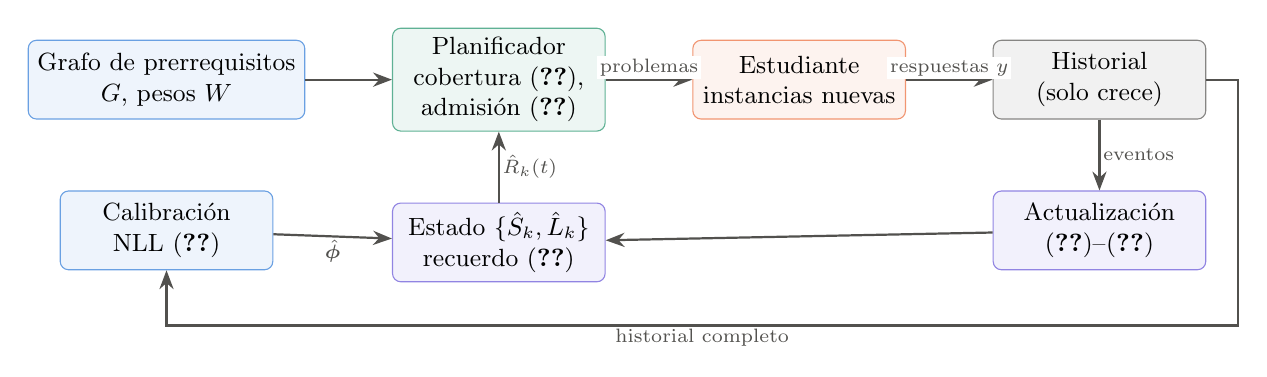
\begin{tikzpicture}[font=\small,
  box/.style={draw=#1!70, fill=#1!8, rounded corners=3pt, minimum height=10mm, minimum width=27mm, align=center},
  ar/.style={-{Stealth[length=2.4mm]}, thick, cg},
  lb/.style={font=\scriptsize, text=cg, fill=white, inner sep=1pt}]
\node[box=c1] (g) {Grafo de prerrequisitos\\$G$, pesos $W$};
\node[box=c3, right=11mm of g] (p) {Planificador\\cobertura \eqref{eq:cobertura},\\admisión \eqref{eq:admision}};
\node[box=c2, right=11mm of p] (s) {Estudiante\\instancias nuevas};
\node[box=cg, right=11mm of s] (h) {Historial\\(solo crece)};
\node[box=c4, below=9mm of p] (st) {Estado $\{\Sh_k,\Lh_k\}$\\recuerdo \eqref{eq:mem}};
\node[box=c4, below=9mm of h] (u) {Actualización\\\eqref{eq:acierto}--\eqref{eq:fallo}};
\node[box=c1, below=9mm of g] (c) {Calibración\\NLL \eqref{eq:nll}};
\draw[ar] (g) -- (p);
\draw[ar] (p) -- node[lb,above]{problemas} (s);
\draw[ar] (s) -- node[lb,above]{respuestas $y$} (h);
\draw[ar] (h) -- node[lb,right]{eventos} (u);
\draw[ar] (u) -- (st);
\draw[ar] (st) -- node[lb,right]{$\Rh_k(t)$} (p);
\draw[ar] (h.east) -- ++(4mm,0) |- node[lb,below,pos=0.75]{historial completo} ($(c.south)+(0,-7mm)$) -- (c.south);
\draw[ar] (c) -- node[lb,below]{$\hat{\bm\phi}$} (st);
\end{tikzpicture}}
\Description{Diagrama de bloques. El grafo de prerrequisitos alimenta al planificador, que envía problemas al estudiante. Las respuestas se agregan al historial, que dispara la actualización del estado; el estado devuelve al planificador las estimaciones de recuerdo. El historial completo alimenta también la calibración, cuyos parámetros alimentan al estado.}
\caption{Ciclo diario del sistema. El estado es siempre una reproducción del historial, que solo crece, con los parámetros vigentes; así el modelo puede recalibrarse sin perder información.}
\label{fig:ciclo}
\end{figure}

%=====================================================================
\section{Estudio de simulación}
\label{sec:sim}
%=====================================================================

Evaluar el planificador con el mismo modelo que genera los datos garantizaría el éxito por construcción. Por eso el simulador separa la \emph{verdad} (cómo aprende y olvida el estudiante simulado, que el planificador nunca ve) del \emph{modelo} de las secciones~\ref{sec:modelo} y~\ref{sec:planificador}, y especifica mal el segundo a propósito (Tabla~\ref{tab:verdad}).

\begin{table}[t]
\centering
\caption{Diferencias deliberadas entre el estudiante simulado y el modelo del planificador.}
\label{tab:verdad}
\setlength{\tabcolsep}{4pt}
\begin{tabularx}{\textwidth}{@{}l>{\raggedright\arraybackslash}X>{\raggedright\arraybackslash}X@{}}
\toprule
& Verdad (estudiante simulado) & Modelo (planificador) \\
\midrule
Olvido & ley de potencia $R=(1+F\Delta t/S)^{C}$ & exponencial \eqref{eq:mem} \\
Ganancia & tipo FSRS, $\gamma S^{-b}(e^{c(1-R)}-1)$ & $G(1-\Rh)$ \eqref{eq:acierto} \\
Fallo & lapso solo en los componentes no recuperados & culpa repartida \eqref{eq:culpa} \\
Bases débiles & según el escenario (A o B) & solo la compuerta de admisión \\
Heterogeneidad & habilidad latente $\theta_i\sim N(0,0.35^2)$ & ninguna \\
\bottomrule
\end{tabularx}
\end{table}

\paragraph{Estudiante simulado.} El estudiante $i$ tiene una habilidad latente $\theta_i$. Sea $\tilde d_k$ la profundidad de la habilidad $k$ en el grafo, reescalada para que la habilidad más profunda tenga profundidad 6 en los grafos de subtemas. La estabilidad inicial es $S^0_{ik}=S_0e^{\theta_i-\delta\tilde d_k}$ y la escala de ganancia es $\gamma_{ik}=e^{a+0.5\theta_i-0.1\tilde d_k}$. El recuerdo verdadero sigue la ley de potencia de FSRS, $R_k(t)=(1+F\,(t-L_k)/S_k)^{C}$ con $F=19/81$ y $C=-0.5$, de modo que $S$ es el número de días hasta que el recuerdo cae a 0.9. Al introducir una habilidad, su estabilidad es $S^0_{ik}\prod_{p\in\Pre(k)}r_p^{\,w_{\mathrm{pre}}}$ (con piso $\Smin$), donde $r_p=R_p(t)$ en el escenario~A y $r_p=R_p(t)(1-e^{-S_p/\kappa})$ en el~B. En un intento, cada componente se recupera con probabilidad $R_k^{\,w_{jk}}$; la respuesta es correcta con probabilidad $1-s$ si se recuperaron todos y con probabilidad $g$ en otro caso. La memoria cambia según lo que \emph{realmente} se recuperó: un componente recuperado gana $S_k\leftarrow S_k[1+w_{jk}c_k\gamma_{ik}S_k^{-b}(e^{c(1-R_k)}-1)]$ y uno no recuperado sufre un lapso, $S_k\leftarrow\max(\Smin,S_k(1-\ell w_{jk}))$. En el escenario~B, $c_k=\prod_{p\in\Pre(k)}(1-e^{-S_p/\kappa})^{w_{\mathrm{pre}}}$, de modo que los repasos de una habilidad consolidan menos mientras sus prerrequisitos sigan frágiles; en el~A, $c_k=1$. Usamos $S_0=0.6$ días, $\delta=0.15$, $a=\ln4$, $b=0.15$, $c=2$, $\ell=0.6$, $\kappa=4$ días, $s=0.05$, $g=0.02$ y $\Smin=0.2$ días.

\paragraph{Dominio.} Usamos un grafo de prerrequisitos de mecánica clásica de bachillerato en dos niveles de granularidad. El grafo de \emph{unidades} tiene 15 unidades agrupadas en siete áreas (bases matemáticas, cinemática, dinámica, cantidad de movimiento, trabajo y energía, sistemas y rotación) y 26 aristas, con profundidad máxima 8. El grafo de \emph{subtemas} tiene 168 subtemas de esas unidades (por ejemplo, «alcance horizontal» o «fuerza de fricción cinética») y 279 dependencias anotadas a mano, con profundidad máxima 20. Como control estructural, la variante \emph{lineal} sustituye las dependencias explícitas por cadenas: cada unidad se convierte en una secuencia de sus subtemas, y cada arista entre unidades une el último subtema de la unidad de origen con el primero de la de destino (profundidad máxima 103).

\paragraph{Políticas.} \emph{Propuesta}, con $\rstar=0.7$, $r_{\min}=0.6$, $\Slisto=7$ días, $\rho=0.8$ y $w_{\mathrm{pre}}=0.5$; también con $\rstar=0.9$, y cuatro ablaciones: sin crédito a prerrequisitos ($w_{\mathrm{pre}}=0$ en el modelo), sin culpa bayesiana ($b_k=1$), sin control de carga y sin compuerta de prerrequisitos. \emph{Anki SM-2}: una tarjeta por tema, introducidas en el orden del libro hasta $m_{\max}$ por día, con intervalos $1$, $6$, $I\cdot E$ y facilidad inicial $E=2.5$. \emph{Libro bloqueado}: temas en el orden del libro, sin repaso. \emph{Libro con repaso acumulativo}: lo mismo, pero 2 de los $U$ problemas de cada sesión se toman al azar de temas anteriores. Todas las políticas reciben el mismo número de problemas por sesión.

\paragraph{Protocolo y métrica.} El curso dura 12 semanas con cinco sesiones por semana (60 sesiones). El grafo de unidades usa $U=6$, $n_{\mathrm{intro}}=3$ y $m_{\max}=1$; los de subtemas, $U=10$, $n_{\mathrm{intro}}=2$ y $m_{\max}=3$. La métrica principal es la media, sobre \emph{todas} las habilidades del grafo, de la probabilidad de que el estudiante resuelva un problema nuevo de cada una 30 días después de la última sesión, sin práctica intermedia. Una habilidad no introducida cuenta como $g=0.02$, así que la métrica premia tanto la retención como la cobertura. Cada política se aplica a los mismos 300 estudiantes simulados y las diferencias se emparejan por estudiante. Los parámetros $\bm\phi$ se estiman en cada escenario con un piloto simulado de 100 estudiantes distintos, en el que los temas se introducen en el orden del libro y se repasan en momentos aleatorios.

%=====================================================================
\section{Resultados}
\label{sec:resultados}
%=====================================================================

\paragraph{Grafo de unidades: presupuesto holgado.} Con 15 unidades y 60 sesiones hay cuatro sesiones por tema, y todas las políticas introducen el temario completo. Cualquier política espaciada supera al libro bloqueado por 0.28--0.29, pero el planificador propuesto (0.743 en el escenario~A y 0.714 en el~B) no supera a Anki SM-2 (0.749 y 0.722); la compuerta de prerrequisitos le cuesta 0.009--0.011 porque retrasa las introducciones en un grafo profundo. Solo con un presupuesto escaso ($U=4$) aparece una ventaja pequeña: 0.731 frente a 0.714 en~A y 0.695 frente a 0.681 en~B. Las estimaciones del piloto fueron $\Sh_0=5.23$, $G=6.07$ y $\lambda=0.09$ en~A.

\paragraph{Grafo de subtemas: presupuesto escaso.} Con 168 subtemas ninguna política adaptativa introduce el temario completo, y el panorama cambia (Tabla~\ref{tab:sub} y Fig.~\ref{fig:barras}). Las estimaciones del piloto fueron $\Sh_0=8.2$, $G=7.2$ y $\lambda=0.13$ en~A. El planificador propuesto supera a Anki por $+0.090$ en~A y $+0.047$ en~B, y la ventaja se mantiene con $U\in\{6,10,14\}$. El mecanismo es la cobertura: Anki acumula repasos vencidos y deja de introducir temas (71 frente a 106 en~A y 63 frente a 79 en~B). El crédito a prerrequisitos aporta $+0.014$ en~A, porque un problema avanzado repasa varios subtemas cuando los lugares escasean; la compuerta aporta $+0.015$ en~B, donde aprender sobre bases frágiles causa un daño persistente; la culpa bayesiana aporta solo entre $+0.002$ y $+0.004$. Quitar el control de carga \emph{mejora} la métrica en $+0.027$, a costa de más temas con menos retención, de modo que, con esta métrica, la restricción de carga es conservadora.

\begin{table}[t]
\centering
\caption{Grafo de subtemas (168 nodos, $U=10$). Prueba diferida (media por estudiante), diferencia pareada respecto al planificador propuesto, temas introducidos y número de subtemas con $P\ge0.8$. Los intervalos de confianza del 95\,\% de las diferencias son de aproximadamente $\pm0.002$.}
\label{tab:sub}
\setlength{\tabcolsep}{3pt}
\begin{tabular}{@{}lcccccccc@{}}
\toprule
& \multicolumn{4}{c}{A: efecto leve} & \multicolumn{4}{c}{B: efecto persistente} \\
\cmidrule(lr){2-5}\cmidrule(lr){6-9}
Política & Prueba & $\Delta$ & Temas & $P\!\ge\!0.8$ & Prueba & $\Delta$ & Temas & $P\!\ge\!0.8$ \\
\midrule
Propuesta ($\rstar=0.7$) & 0.370 & --- & 106 & 5.5 & 0.285 & --- & 79 & 7.1 \\
Propuesta ($\rstar=0.9$) & 0.239 & $-0.131$ & 56 & 12.6 & 0.189 & $-0.097$ & 42 & 13.1 \\
\quad sin crédito a prerreq. & 0.355 & $-0.014$ & 98 & 8.2 & 0.282 & $-0.003$ & 74 & 9.6 \\
\quad sin culpa bayesiana & 0.366 & $-0.004$ & 103 & 6.3 & 0.283 & $-0.002$ & 78 & 7.3 \\
\quad sin control de carga & 0.397 & $+0.027$ & 134 & 2.3 & 0.312 & $+0.026$ & 101 & 3.2 \\
\quad sin compuerta & 0.372 & $+0.002$ & 108 & 4.9 & 0.270 & $-0.015$ & 79 & 6.5 \\
Anki SM-2 & 0.280 & $-0.090$ & 71 & 11.0 & 0.239 & $-0.047$ & 63 & 8.5 \\
Libro + repaso & 0.275 & $-0.095$ & 168 & 1.6 & 0.144 & $-0.142$ & 168 & 1.1 \\
Libro bloqueado & 0.167 & $-0.203$ & 168 & 0.0 & 0.078 & $-0.207$ & 168 & 0.0 \\
\bottomrule
\end{tabular}
\end{table}

\begin{figure}[t]
\centering
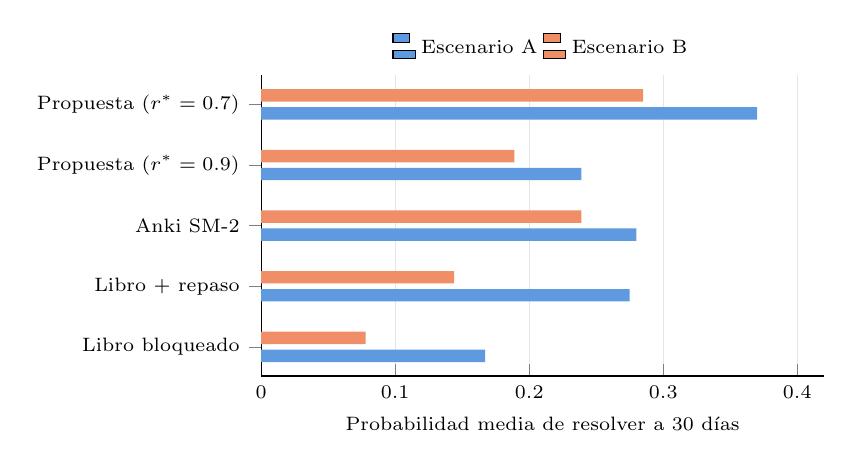
\begin{tikzpicture}
\begin{axis}[
  xbar, width=0.72\textwidth, height=5.4cm, bar width=4.5pt,
  enlarge y limits=0.12, xmin=0, xmax=0.42,
  xlabel={Probabilidad media de resolver a 30 días},
  symbolic y coords={bt,tr,anki,p9,p7},
  yticklabels={Libro bloqueado,Libro + repaso,Anki SM-2,Propuesta ($r^*=0.9$),Propuesta ($r^*=0.7$)},
  ytick=data, tick label style={font=\scriptsize}, label style={font=\scriptsize},
  x tick label style={/pgf/number format/fixed},
  legend style={at={(0.5,1.02)},anchor=south,legend columns=2,font=\scriptsize,draw=none},
  axis lines*=left, xmajorgrids, grid style={gray!20}]
\addplot[fill=c1!75, draw=none] coordinates {(0.167,bt) (0.275,tr) (0.280,anki) (0.239,p9) (0.370,p7)};
\addplot[fill=c2!75, draw=none] coordinates {(0.078,bt) (0.144,tr) (0.239,anki) (0.189,p9) (0.285,p7)};
\legend{Escenario A, Escenario B}
\end{axis}
\end{tikzpicture}
\Description{Gráfica de barras horizontales de la prueba diferida por política y escenario en el grafo de subtemas. La política propuesta con retención objetivo 0.7 tiene las barras más largas en ambos escenarios (0.370 y 0.285), seguida de Anki SM-2 (0.280 y 0.239); el libro bloqueado tiene las más cortas (0.167 y 0.078).}
\caption{Prueba diferida en el grafo de subtemas, por política y escenario (datos de la Tabla~\ref{tab:sub}).}
\label{fig:barras}
\end{figure}

\paragraph{Cobertura frente a retención.} La métrica mezcla dos cantidades. Si se descuenta la contribución $g$ de los temas no introducidos, la probabilidad media \emph{sobre los temas introducidos} es de alrededor de 0.58 con el planificador propuesto, 0.64 con Anki y 0.68 con el propuesto con $\rstar=0.9$ en~A (0.58 y 0.60 para los dos primeros en~B). La columna $P\ge0.8$ dice lo mismo: Anki y la variante con $\rstar=0.9$ dejan más subtemas «dominados». El planificador con $\rstar=0.7$ gana porque cubre más temas con una retención algo menor por tema. Bajar todavía más $\rstar$ mejora la métrica (0.403 con $\rstar=0.5$ en~A), mientras que $\rstar\ge0.9$ la deteriora mucho: repasar con $\Rh\approx0.9$ rinde poco bajo la dinámica verdadera, y la carga estimada~\eqref{eq:carga} se infla y bloquea la admisión. La elección de $\rstar$ es, por lo tanto, una decisión pedagógica sobre esta frontera, no un detalle técnico.

\paragraph{La estructura del grafo importa.} En la variante lineal, la ventaja sobre Anki en el escenario~A se reduce de $+0.090$ a $+0.012$ (0.298 frente a 0.286). En el escenario~B, el planificador propuesto cae a 0.124, por debajo del 0.238 de Anki: con 103 niveles solo hay un tema admisible a la vez, y la compuerta deja al sistema con 28 temas en todo el curso. Anki, que ignora el grafo, no se ve afectado. Un grafo con dependencias falsas castiga justamente al planificador que lo respeta. Una advertencia: el reescalado de la profundidad difiere entre los dos grafos, así que la comparación también cambia la dificultad relativa de los temas en la verdad.

\paragraph{Calibración.} Fuera de muestra, sobre los intentos generados por la política propuesta, el modelo exponencial obtiene un AUC de 0.67 y un puntaje de Brier de 0.17--0.18 en el grafo de subtemas (AUC de 0.66--0.70 en el de unidades), y sobreestima la probabilidad de acierto en el rango medio. Es lo esperable, porque la verdad usa olvido de ley de potencia y lapsos ocultos. El planificador funciona razonablemente bien pese a la mala especificación, y la calibración es el diagnóstico natural para detectarla con datos reales.

%=====================================================================
\section{Discusión y limitaciones}
%=====================================================================

En todas las condiciones, el efecto más grande y robusto es espaciar frente a la enseñanza bloqueada ($+0.20$ a $+0.29$). Entre políticas espaciadas, el modelo propuesto ayuda solo cuando se cumplen dos condiciones: el grafo es de grano fino en relación con el presupuesto de práctica, y sus dependencias son reales. Sus componentes más finos (culpa bayesiana, crédito a prerrequisitos y compuerta) tienen efectos pequeños y dependientes del escenario; el mecanismo dominante es que la admisión con control de carga sigue introduciendo temas cuando un planificador de tarjetas se atasca. Estos hallazgos coinciden con la advertencia del marco KLI de que la granularidad es una cuestión empírica \cite{koedinger2012}, y hacen que validar el grafo de prerrequisitos sea tan importante como la regla de repaso.

El estudio tiene limitaciones claras. (i) La verdad es también un modelo: los resultados indican qué componentes \emph{podrían} importar y bajo qué supuestos, no cuánto ganaría un aula. (ii) El valor $\rstar=0.7$ se eligió tras un barrido preliminar que usó la verdad; debe fijarse con un procedimiento que no la use, por ejemplo optimizándolo en simulación con el modelo ajustado a datos de un piloto. (iii) La métrica favorece la cobertura, y un $\rstar$ bajo implica más fallos durante la práctica, con posibles costos de motivación que no se modelan. (iv) Las 279 dependencias entre subtemas son un borrador anotado a mano, pendiente de validación docente. (v) El modelo fija $s$ y $g$, usa la regla simple de culpa y no tiene efectos por estudiante ni por habilidad; en la variante lineal del escenario~B, la estimación $\hat\lambda\approx0$ sugiere problemas de identificabilidad. (vi) No se modelan la práctica intercalada, la fatiga, el abandono ni la variación entre instancias de un mismo tipo de problema \cite{rohrer2015}.

%=====================================================================
\section{Conclusiones y trabajo futuro}
%=====================================================================

Extendimos la dinámica de memoria de MEMORIZE a habilidades procedimentales relacionadas por prerrequisitos, con crédito fraccional, culpa bayesiana, admisión con control de carga y un planificador submodular con garantía de $1-1/e$. En simulación sobre mecánica de bachillerato, el planificador supera a SM-2 en un grafo de grano fino con presupuesto escaso, sobre todo por cobertura, y las dependencias falsas lo perjudican. Ya existe un prototipo web que implementa el modelo sobre 13 subtemas de cinemática con 33 plantillas paramétricas. Los siguientes pasos son: un piloto de calibración con intervalos de repaso aleatorios para estimar los parámetros, contrastar la matriz $Q$ fraccional contra habilidades independientes y comparar el olvido exponencial con la ley de potencia; un modelo jerárquico con efectos por estudiante y por habilidad; la validación docente del grafo; y un experimento intrasujeto contrabalanceado en el aula, al estilo de Lindsey y colaboradores \cite{lindsey2014}, que compare el planificador con SM-2 o FSRS con el mismo tiempo de práctica y una prueba diferida a 30 días con problemas nuevos. Con diferencias pareadas, $\alpha=0.05$ y potencia de 0.8, la muestra necesaria es $n\approx7.85/d_z^2$: 32 estudiantes para $d_z=0.5$ y 88 para $d_z=0.3$.

\begin{credits}
\subsubsection{\discintname}
Los autores declaran que no tienen conflictos de interés relacionados con el contenido de este artículo.
\end{credits}

\bibliographystyle{splncs04}
\bibliography{refs}

\end{document}
